\section{Spectral filter on graph}

In this section we introduce spectral filtering of signals defined over a graph. 

\subsection{Spectral domain}

For a graph $G = (V, E, W)$ with Laplacian $L \in \R^{n\times n}$, we have the following spectral decomposition, with $U \in \R^{n\times n}$ the change of basis matrix that diagonalizes the Laplacian $L$:
%
\begin{equation}
    L = U \Lambda U^T \quad \mathrm{with} \quad \Lambda = \mathrm{diag}([\lambda_0, \dots, \lambda_{n-1}])
\end{equation}
%
The authors then introduce the Graph Fourier Transform (GFT) which takes a spatial one-dimensional signal (defined on the nodes of G) $x \in \R^n$ and maps it to its counterpart in the spectral domain $\hat x = U^T x \in \R^n$. The inverse operation $x = U \hat x$, allows to switch between the spatial on spectral domain at ease, provided the Fourier basis $U$ is known.

On figure \ref{fig:fourier_modes} we can see plots of some of the Laplacian eigenvectors over a regular 2D grid graph. We can see that those Fourier modes define complex periodic patterns, that shows quite clearly why the Laplacian eigendecomposition can be used as a Graph Fourier Transform.

\begin{figure}
    \centering
    \subfigure[mode 91]{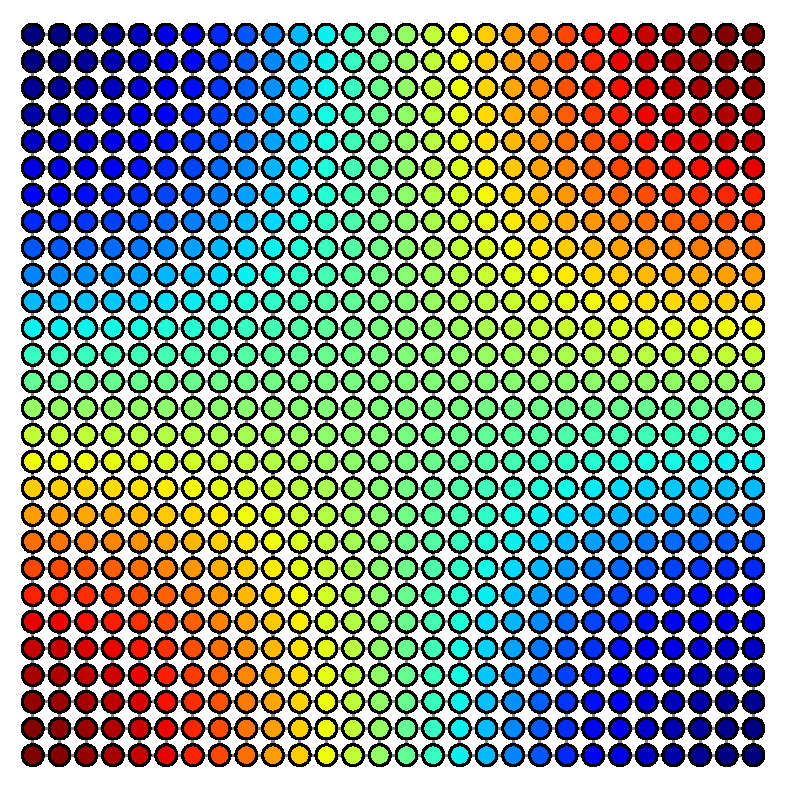
\includegraphics[width=0.24\textwidth]{img/mode3.pdf}}
    \subfigure[mode 215]{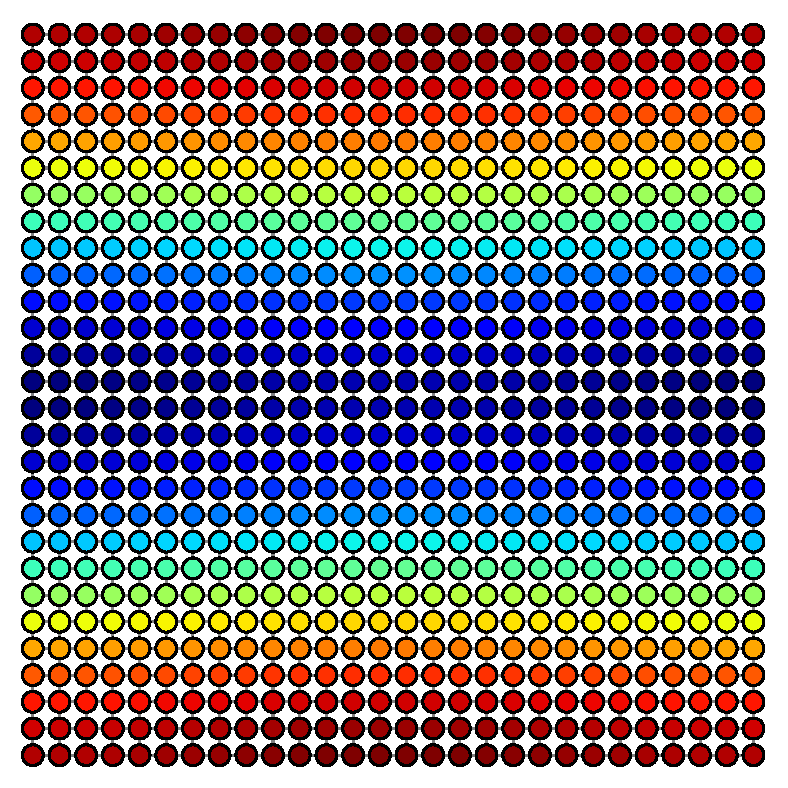
\includegraphics[width=0.24\textwidth]{img/mode5.pdf}}
    \subfigure[mode 474]{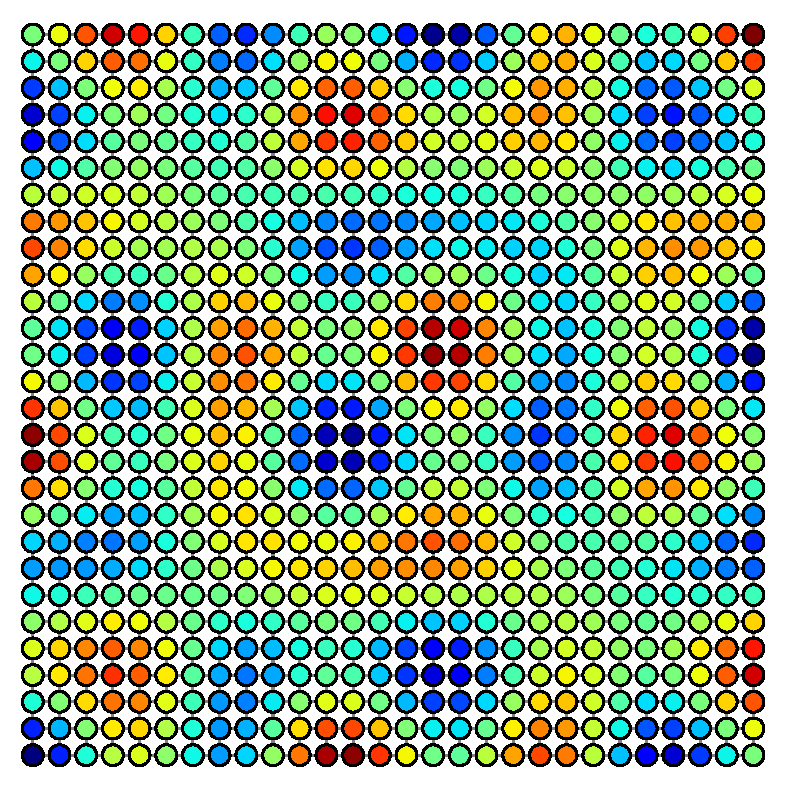
\includegraphics[width=0.24\textwidth]{img/mode50.pdf}}
    \subfigure[mode 613]{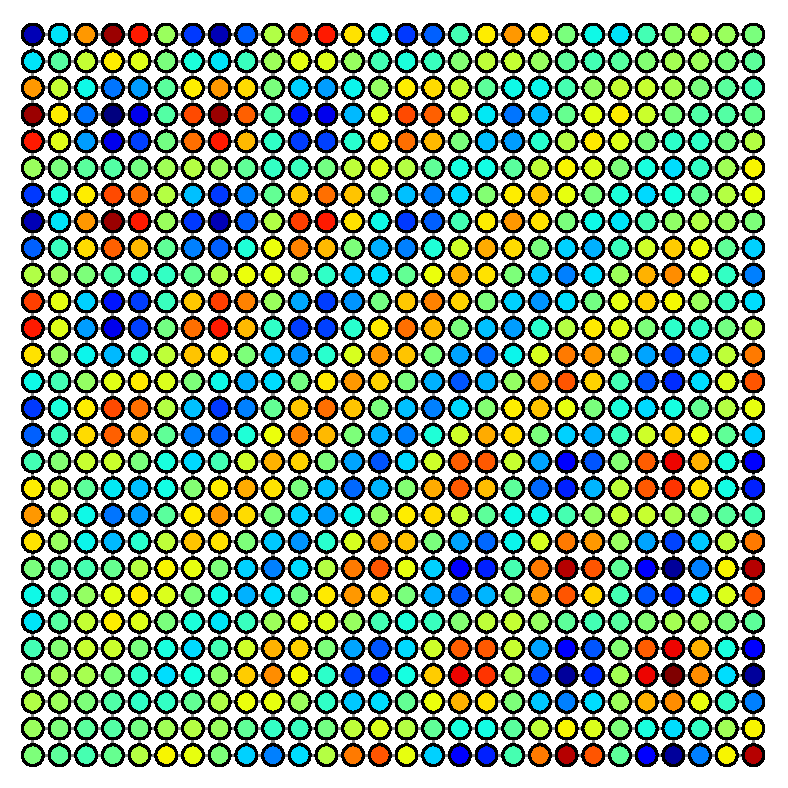
\includegraphics[width=0.24\textwidth]{img/mode100.pdf}}
    \caption{Some Fourier Modes plotted over the graph (i.e. Laplacian eigenvectors)}
    \label{fig:fourier_modes}
\end{figure}


\subsection{Filtering}

Applying a filter in the spatial domain amounts to perform an element-wise product in the spectral domain. Hence we can take a filter operator $g_\theta(.)$ that is defined in the spectral domain (and depends on some parameter vector $\theta$) and apply it to $\bar x$: the output in the spectral domain is then $\bar y = g_\theta \bar x = g_\theta U^T x$. To get the final filtered signal $y$ we go back to the spatial domain using the inverse GFT:
%
\begin{equation}
    y = U \bar y = U g_\theta  U^T x
\end{equation}
%
In practice the element wise product of $U^T x$ by all the components of the filter $g_\theta$ can be achieved as a matrix multiplication if we define our filter as a diagonal matrix in $\R^{n\times n}$. It follows that any filter is of the form $\mathrm{diag}(\theta)$ with $\theta \in \R^n$. The authors refer to this general construction as a \textit{non-parametric filter} because it has the maximum allowed degrees of freedom.

\subsection{Localized filters}

As pointed out by the authors, this general formulation is not satisfactory because it is not localized in space (each component of the output signal depends on every component of the input signal) and the number of parameters to learn is equal to the signal size which is a bottleneck and is not the case for standard convolutional filters on images.\\

One can show \cite{hammond2011wavelets} that if the shortest path between two vertices $i$ and $j$ on the graph is strictly greater than $K$ then $(L^K)_{i,j} = 0$. A natural idea that then arises is to design a filter that is parametrized over powers of the Laplacian (or in the spectral domain, the powers of $\Lambda$) to control the spatial localization of the filter:
%
\begin{equation}
    g_\theta(\Lambda) = \sum_{k=0}^{K-1} \theta_k \Lambda^k \label{eq:localized_filter}
\end{equation}
%
Thus using the previously stated property it is easy to prove the spatial $K-$localization of such filters (see the original paper). In addition the learning complexity is now independent of the signal size since we only have $K$ parameters. 

Figure \ref{fig:filtered} shows an MNIST "9" sample filtered using different powers of the Laplacian. We can see that depending on K, only some large areas of stationary signals are kept, while the rest is discarded from the representation.

\begin{figure}
    \centering
    \subfigure[$\Lambda^1$]{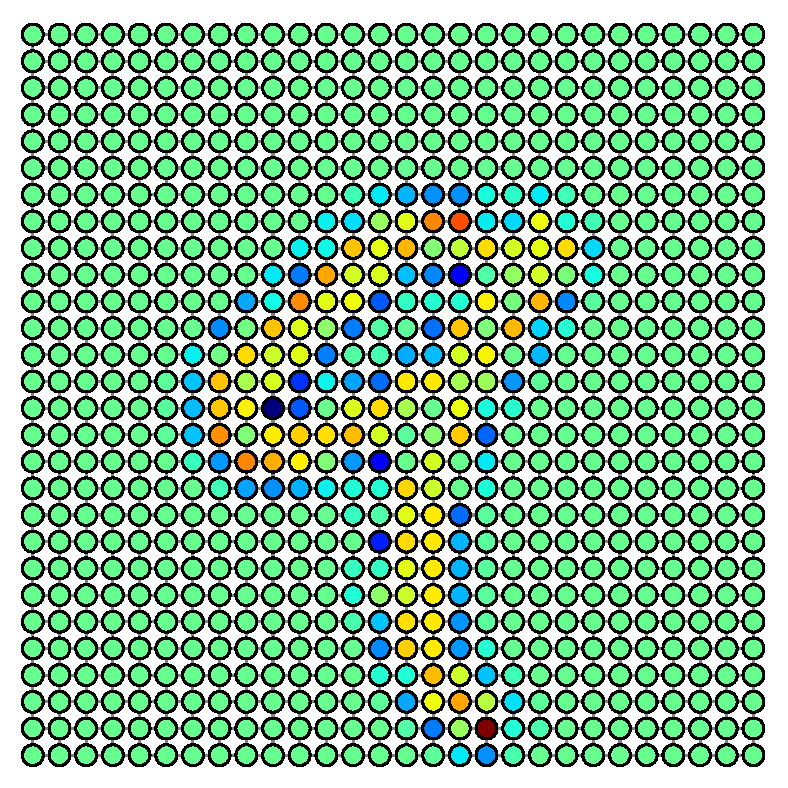
\includegraphics[width=0.24\textwidth]{img/L1.pdf}}
    \subfigure[$\Lambda^3$]{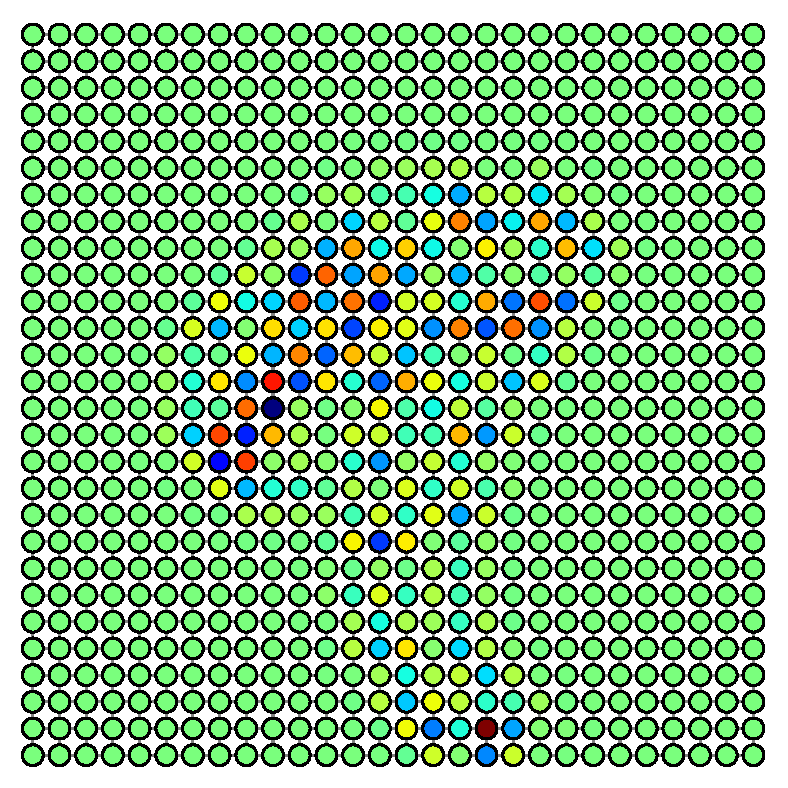
\includegraphics[width=0.24\textwidth]{img/L3.pdf}}
    \subfigure[$\Lambda^5$]{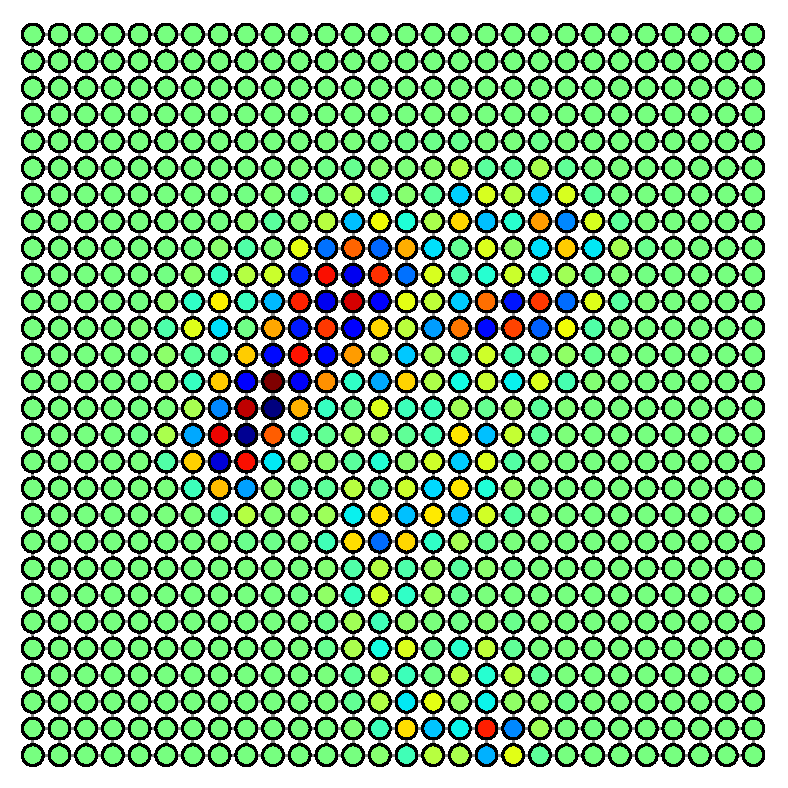
\includegraphics[width=0.24\textwidth]{img/L5.pdf}}
    \subfigure[$\Lambda^9$]{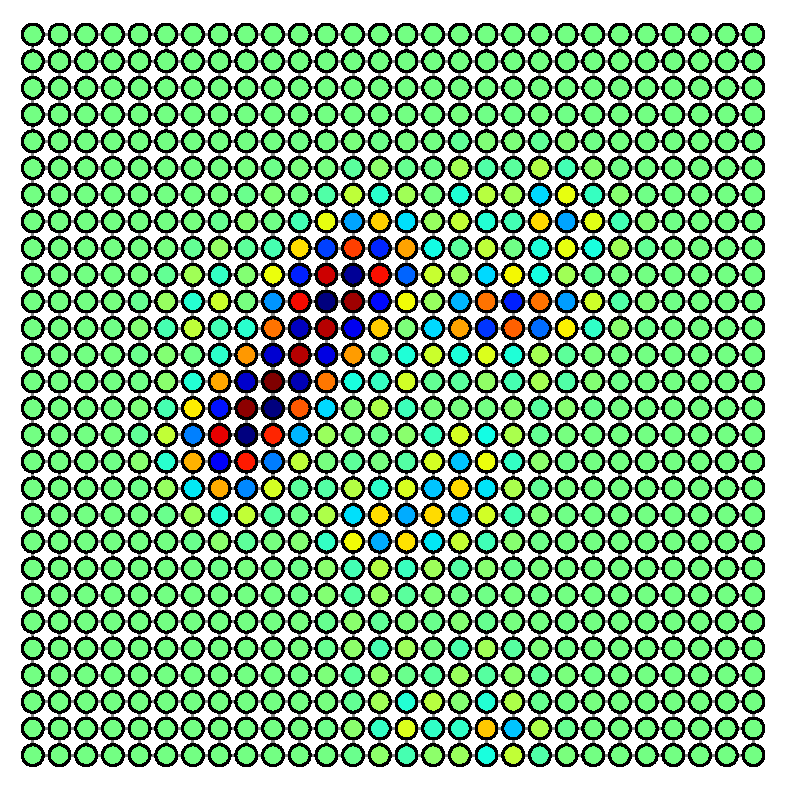
\includegraphics[width=0.24\textwidth]{img/L8.pdf}}
    \caption{Localized filtering of a signal using different powers of $\Lambda$.}
    \label{fig:filtered}
\end{figure}

\subsection{Fast filtering or Chebyshev approximated filters}
%
Equation \ref{eq:localized_filter} is the theoretical key to construct a CNN on a graph, but for an efficient implementation it has one downside: in practice switching between the spatial and the spectral domain implies two matrix multiplications by $U^T$ and $U$ (which are dense matrices) and has a cost $\mathcal{O}(n^2)$. The authors, thus, make use of the Chebyshev polynomial approximation $T_k(x)$ defined recursively by $T_k(x) = 2xT_{k-1}(x) - T_{k-2}(x)$ with $T_0=1$ and $T_1 = x$ which forms an orthogonal basis of $L^2([-1,1])$ with respect to the weights $1/\sqrt{1 - x^2}$. The proposed filter is then defined as:
\begin{equation}
    g_\theta(\Lambda) = \sum_{k=0}^{K-1} \theta_k T_k(\tilde \Lambda) \label{eq:localized_filter}
\end{equation}
%
Where $\tilde \Lambda = 2\Lambda / \lambda_max - I_n$ is the scaled diagonalized Laplacian whose coefficients lie in $[-1, 1]$. Because each $T_k$ has degree $k$, this is a re-parametrization of equation \ref{eq:localized_filter} which proves directly the spatial localization. Finally the authors explicit the output signal y as $y = g_\theta(L)x = \sum_{k=0}^{K-1} \bar x_k$ with $\bar x_k = \theta_k T_k(\tilde L) x$. The $\bar x_k$'s can be computed by the recursion $\bar x_k = 2 \tilde L \bar x_{k-1} - \bar x_{k-2}$ with $\bar x_0 = x$ and $\bar x_1 = \tilde L x$. The filtered signal is then given by $y = [\bar x_0, \dots, \bar x_{K-1}]\theta$ and the filtering cost is $\mathcal{O}(K|E|)$ because the matrix products during the recursion involve a sparse matrix (the scaled Laplacian) and dense vectors. Algorithm \ref{alg:filtering} summarizes how to perform the filtering. \footnote{Our implementation doesn't benefit from the Laplacian sparsity since our goal was just to demonstrate our understanding of CNN on graphs and not to produce scalable code.}\\

\begin{algorithm}[ht]
 \KwData{input signal $x \in \R^d$, filter parameters $\theta \in \R^K$ , Graph Laplacian $L_\mathcal{G} \in \R^{d \times d}$}
 \KwResult{filtered signal $y \in \R^d $}
 
 \textbf{Initialization:}\\
    $\tilde{L} = 2 L / \lambda_{max} - I_d$ \\
    $\bar{x}_0 = x$ \\
    $\bar{x}_1 = \tilde{L}x$
 
 \For{$k=2$ to $K-1$}{
    $\bar{x}_k=2\tilde{L}\bar{x}_{k-1} - \bar{x}_{k-2}$
 }
 \textbf{Return:} $y = [\bar{x}_0, \ldots, \bar{x}_{K-1}] \theta$
 \caption{Fast localized spectral filter}
 \label{alg:filtering}
\end{algorithm}

\begin{figure}
    \centering
    \subfigure[$T_1$]{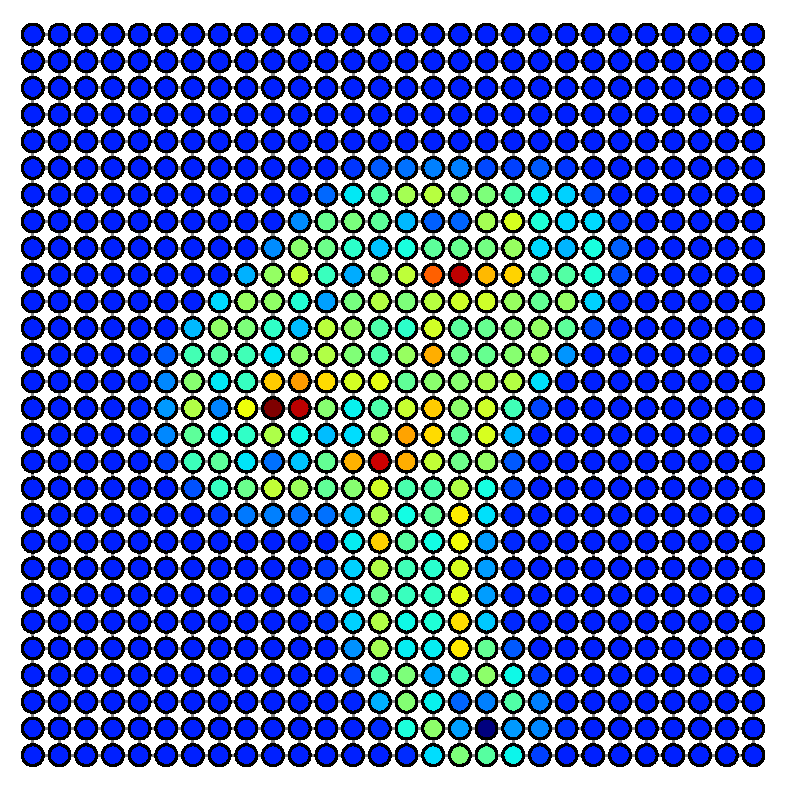
\includegraphics[width=0.24\textwidth]{img/C0.pdf}}
    \subfigure[$T_2$]{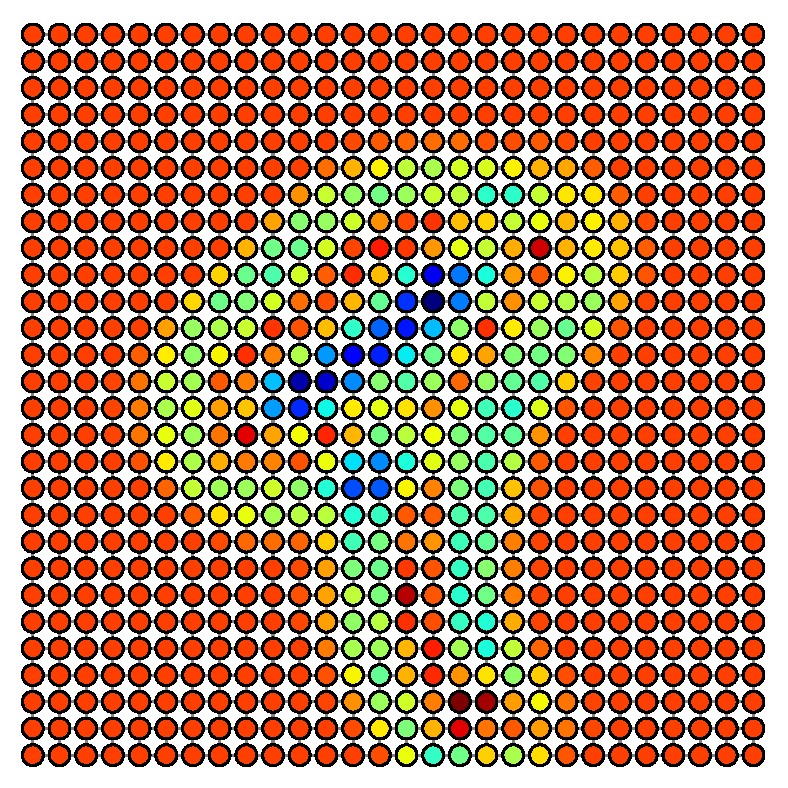
\includegraphics[width=0.24\textwidth]{img/C1.pdf}}
    \subfigure[$T_3$]{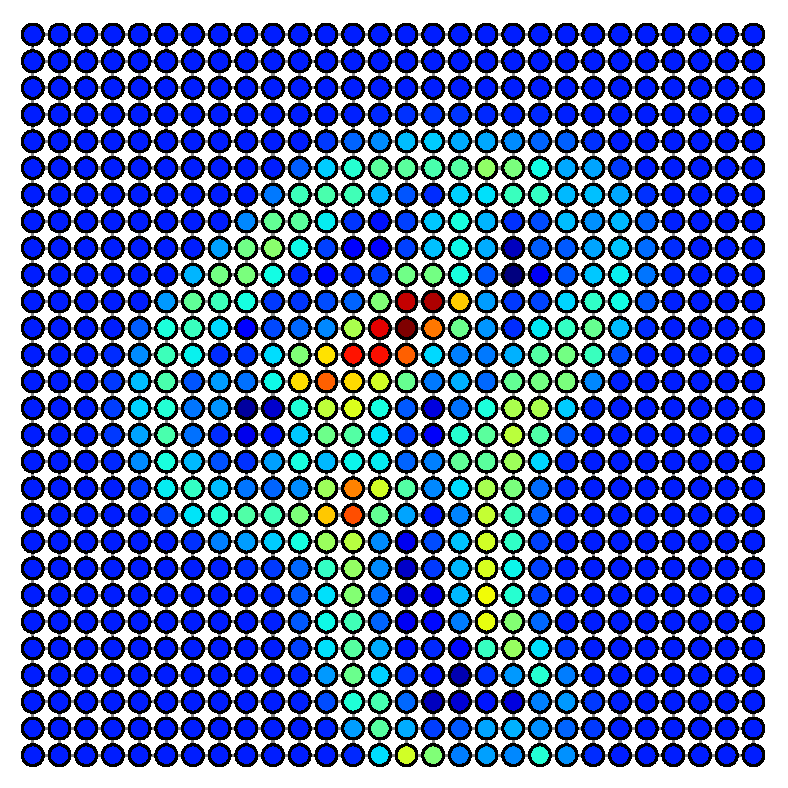
\includegraphics[width=0.24\textwidth]{img/C2.pdf}}
    \subfigure[$T_5$]{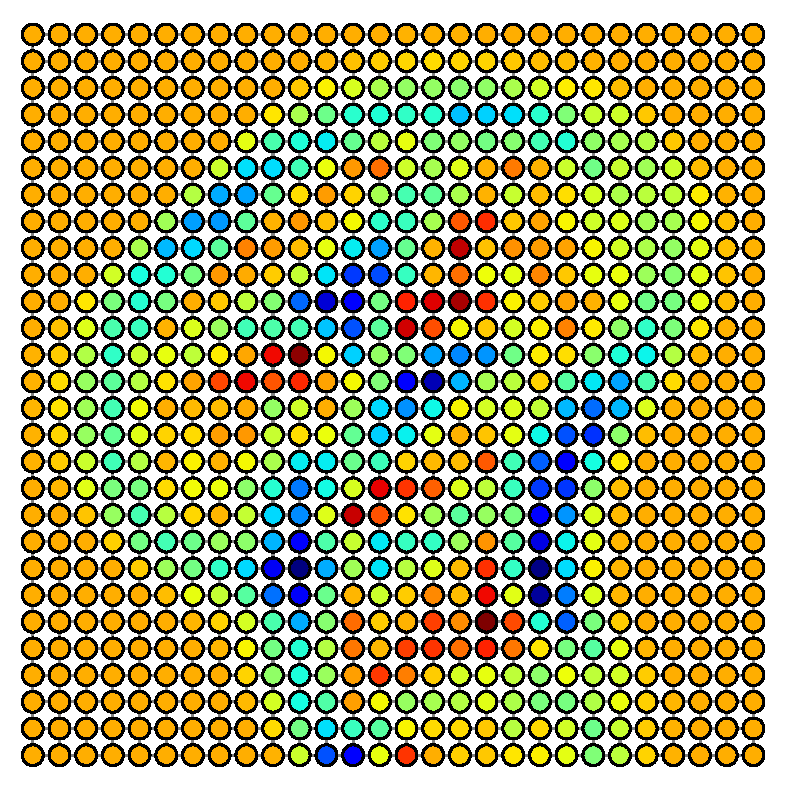
\includegraphics[width=0.24\textwidth]{img/C5.pdf}}
    \caption{Localized filtering of a signal using different orders of Chebyshev approximation.}
    \label{fig:chebyshev_filtered}
\end{figure}

On figure \ref{fig:chebyshev_filtered}, we represented signals filtered using the recursive Chebyshev approximation. The behaviour here is different from the one we had with powers of $\Lambda$, and we can see that the difference formulation of the Chebyshev approximation tends to keep only the boundaries of the signal.

Learning the filters parameters can be achieved using back-propagation and gradient descent (see p.4 of \cite{defferrard2016convolutional} for the gradient expressions). Nevertheless, in our implementation, \texttt{Tensorflow} performs symbolic operations and is able to compute the parameter derivatives automatically which makes it really easy to implement the whole gradient descent even after cascading several filters.\\

An example of filtered signals is given by Figure~\ref{fig:inversed_learnt}: the graph is a grid where each pixel is a node and is connected to its 8 neighbors. On top of this graph the signal is the intensity of each pixel. We randomly chose $K=100$ parameters for a filter and applied it to the signal using the Chebitchev formulation. As expected the filtered signal (left) is blurry. Just to demonstrate the gradient descent using \texttt{Tensorflow}, we tried to retrieve the initial signal (our "9" digit) from the filtered version to see if it is possible to learn an "inverse" filter. After 10~000 iterations of gradient descent, the mean squared error had fallen under 0.04 (i.e. about 20\% average deviation since we normalized the intensity between 0 and 1). The reconstructed signal is far from perfect due to the loss of information during the first filtering but we clearly distinguish the shape of the "9".

\begin{figure}
    \centering
    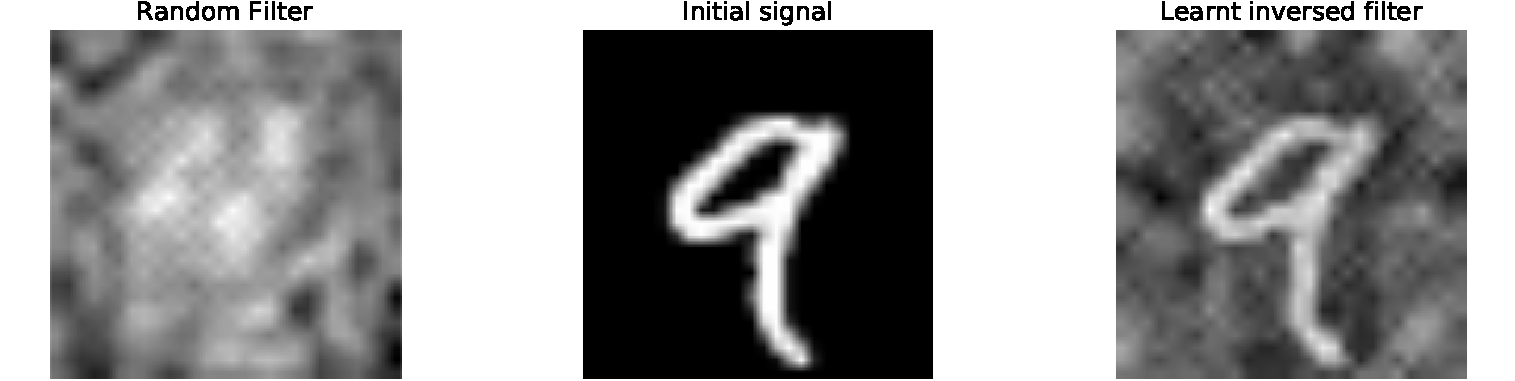
\includegraphics[width=\textwidth]{img/inversed_learnt.pdf}
    \caption{Left: filtered signal with $K=100$ random coefficients. Center: initial signal on the grid graph. Right: filtering of the left signal after having learnt $K=100$ coefficients to create an "inverse" filter using gradient descent.}
    \label{fig:inversed_learnt}
\end{figure}